% Schematic product-coordinate passages, not numerical DF1b trajectories.
% Representative curves solve d eta/d theta = .65 eta in drawing units.
% The half-amplitude tick localizes counted zeros; it is not a passage event.
% Native size: approximately 108 mm wide, with 10 pt labels.
\begin{figure}[H]
\centering
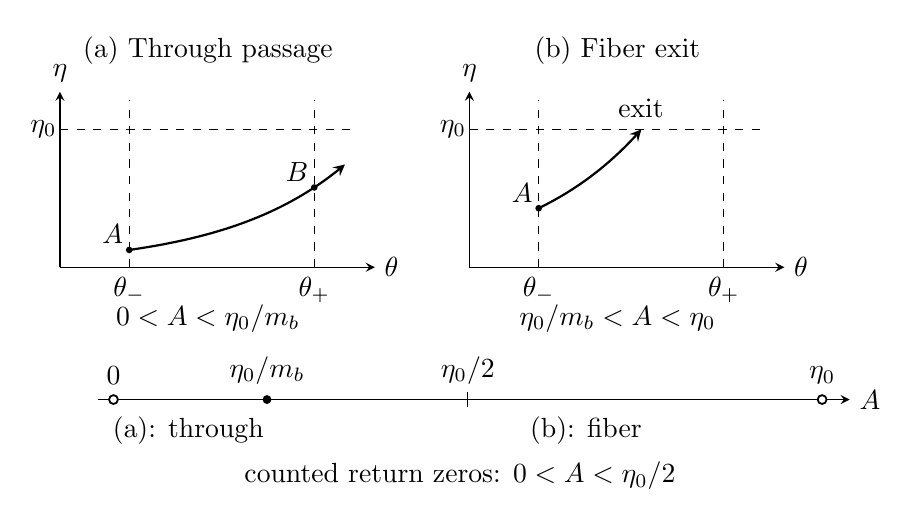
\begin{tikzpicture}[x=10mm,y=10mm,>=stealth,
  every node/.style={font=\fontsize{10}{12}\selectfont},
  axes/.style={->,line width=.45pt},
  section/.style={dashed,line width=.5pt},
  orbit/.style={->,line width=.8pt}]
  \foreach \shift/\panel/\heading in
    {0/a/Through passage,5.2/b/Fiber exit} {
    \begin{scope}[xshift=\shift cm]
      \node at (2,2.75) {(\panel) \heading};
      \draw[axes] (.12,0)--(4.12,0) node[right] {$\theta$};
      \draw[axes] (.12,0)--(.12,2.23) node[above] {$\eta$};
      \draw[section] (1,0)--(1,2.12);
      \draw[section] (3.35,0)--(3.35,2.12);
      \draw[section] (.12,1.75)--(3.83,1.75);
      \node[below] at (1,0) {$\theta_-$};
      \node[below] at (3.35,0) {$\theta_+$};
      \node[left,inner sep=1pt] at (.12,1.75) {$\eta_0$};
    \end{scope}
  }
  \begin{scope}
    \draw[orbit,domain=1:3.74,samples=45,smooth]
      plot (\x,{.22*exp(.65*(\x-1))});
    \fill (1,.22) circle (1.2pt);
    \fill (3.35,{.22*exp(.65*2.35)}) circle (1.2pt);
    \node[above left,inner sep=2pt] at (1,.22) {$A$};
    \node[above left,inner sep=2pt] at (3.35,{.22*exp(.65*2.35)}) {$B$};
    \node at (2,-.65) {$0<A<\eta_0/m_b$};
  \end{scope}
  \begin{scope}[xshift=5.2cm]
    \draw[orbit,domain=1:2.303535169826467,samples=35,smooth]
      plot (\x,{.75*exp(.65*(\x-1))});
    \fill (1,.75) circle (1.2pt);
    \node[above left,inner sep=2pt] at (1,.75) {$A$};
    \node[above,inner sep=2pt] at (2.30,1.82) {exit};
    \node at (2,-.65) {$\eta_0/m_b<A<\eta_0$};
  \end{scope}
  % No-root amplitude order; intersect each branch with the actual image.
  % The filled point is the only possible internal event.
  % The half-amplitude tick and the open outer endpoint are not events.
  \draw[axes] (.6,-1.68)--(10.15,-1.68) node[right] {$A$};
  \draw[fill=white,line width=.65pt] (.8,-1.68) circle (1.6pt);
  \fill (2.75,-1.68) circle (1.6pt);
  \draw[line width=.45pt] (5.3,-1.58)--(5.3,-1.78);
  \draw[fill=white,line width=.65pt] (9.8,-1.68) circle (1.6pt);
  \node[above] at (.8,-1.61) {$0$};
  \node[above] at (2.75,-1.61) {$\eta_0/m_b$};
  \node[above] at (5.3,-1.61) {$\eta_0/2$};
  \node[above] at (9.8,-1.61) {$\eta_0$};
  \node[below] at (1.75,-1.77) {(a): through};
  \node[below] at (6.8,-1.77) {(b): fiber};
  \node at (5.2,-2.65)
    {counted return zeros: $0<A<\eta_0/2$};
\end{tikzpicture}
\caption{Schematic no-root passages in the product coordinates
\eqref{eq:pc-collision-product}. Dashed lines are the fixed bases and exit
level. Trajectory arrows give positive-time direction; the lower line records
increasing $A$. It shows one possible position of the sole seam
$A=\eta_0/m_b$ in $0<A<\eta_0$;
intersect the displayed branch ranges with the actual source image.
Here $m_b>1$ has no uniform upper bound, and the seam or a branch may be
absent from that image. The half-amplitude tick marks localization of
counted return zeros, not a passage event. When a root is present, only
fiber exit remains; $B=m_bA$ is the no-root through relation.}
\label{fig:collision-passages}
\end{figure}
